\documentclass[11pt, dvipsnames, DIV=12]{scrreprt}
\usepackage[english]{babel}

\usepackage[utf8]{inputenc}
\usepackage[T1]{fontenc}
\usepackage{natbib}
\bibliographystyle{abbrvnat}
\usepackage{subcaption}
\usepackage{booktabs}
\usepackage{multirow}
\usepackage{url}
\usepackage{tikz}
\usepackage{paralist}

\usepackage{ifthen}
\newcommand{\CC}[1][]{$\text{C\hspace{-.25ex}}^{_{_{_{++}}}}
\ifthenelse{\equal{#1}{}}{}{\text{\hspace{-.625ex}#1}}$}

\usepackage{bm}
\usepackage{amsmath}
\usepackage{amssymb}
\usepackage{amsthm}
\usepackage{amsfonts}
\usepackage{thmtools}		
\usepackage{mleftright}
\usepackage{stmaryrd}
\usepackage{nicefrac}
\usepackage{algorithm}
\usepackage{algorithmicx}
\usepackage[noend]{algpseudocode}
\renewcommand{\algorithmicrequire}{\textbf{Input:}}
\renewcommand{\algorithmicensure}{\textbf{Output:}}

% Fixes some spacing issues with braces.
\let\originalleft\left
\let\originalright\right
\renewcommand{\left}{\mathopen{}\mathclose\bgroup\originalleft}
\renewcommand{\right}{\aftergroup\egroup\originalright}

\theoremstyle{definition}
\newtheorem{theorem}{Theorem}
\newtheorem{conjecture}{Conjecture}
\newtheorem{proposition}[theorem]{Proposition}
\newtheorem{insight}{Insight}
\newtheorem{observation}{Observation}
\newtheorem{lemma}[theorem]{Lemma}
\newtheorem{corollary}[theorem]{Corollary}
\newtheorem{definition}[theorem]{Definition}
\newtheorem{example}[theorem]{Example}
\newtheorem{remark}[theorem]{Remark}
\newtheorem{claim}[theorem]{Claim}
\newtheorem{fact}[theorem]{Fact}
\usepackage{thm-restate}
\usepackage[mathic=true]{mathtools}
\usepackage{fixmath}
\usepackage{siunitx}

\usepackage{pifont}
\newcommand{\cmark}{\ding{51}}
\newcommand{\xmark}{\ding{55}}
\usepackage{blindtext}

\usepackage{todonotes}

\usepackage{enumitem}
\setlist[enumerate]{itemsep=0.2ex, topsep=0.5\topsep}
\setlist[description]{itemsep=0.2ex, topsep=0.5\topsep}
\setlist[itemize]{itemsep=0.2ex, topsep=0.5\topsep}


% Let cleveref and thmtools work together
\makeatletter
\def\thmt@refnamewithcomma #1#2#3,#4,#5\@nil{%
\@xa\def\csname\thmt@envname #1utorefname\endcsname{#3}%
\ifcsname #2refname\endcsname
\csname #2refname\expandafter\endcsname\expandafter{\thmt@envname}{#3}{#4}%
\fi
}
\makeatother


\usepackage[pagebackref,
pdfa,
hidelinks,
pdftex, 
pdfdisplaydoctitle,
pdfpagelabels,
pdfauthor={},
pdftitle={},
pdfsubject={},
pdfkeywords={},
pdfproducer={Latex with the hyperref package},
pdfcreator={pdflatex}
]{hyperref}

\usepackage[capitalise,noabbrev]{cleveref}   

\usepackage{microtype}
\usepackage{ellipsis}

\usepackage[scaled=0.86]{helvet}
\usepackage{lmodern}

% Bold. 
\newcommand{\mF}{\mathbf{F}}
\newcommand{\mG}{\mathbf{G}}
\newcommand{\mH}{\mathbf{H}}
\newcommand{\mL}{\mathbf{L}}
\newcommand{\mI}{\mathbf{I}}

\newcommand{\mW}{\mathbf{W}}
\newcommand{\ma}{\mathbf{a}}
\newcommand{\mb}{\mathbf{b}}
\newcommand{\mw}{\mathbf{w}}

\newcommand{\ba}{\ensuremath{{\bf a}}}
\newcommand{\bb}{\ensuremath{{\bf b}}}
\newcommand{\bc}{\ensuremath{{\bf c}}}

% Calligraphic.
\newcommand{\cC}{\mathcal{C}}
\newcommand{\cF}{\mathcal{F}}
\newcommand{\cG}{\mathcal{G}}
\newcommand{\cH}{\mathcal{H}}
\newcommand{\cN}{\mathcal{N}}
\newcommand{\cO}{\mathcal{O}}
\newcommand{\cP}{\mathcal{P}}
\newcommand{\cR}{\mathcal{R}}
\newcommand{\cS}{\mathcal{S}}
\newcommand{\cT}{\mathcal{T}}
\newcommand{\cU}{\mathcal{U}}
\newcommand{\cV}{\mathcal{V}}

% Sans serif.
\newcommand{\sC}{\mathsf{C}}

% Blackboard.
\newcommand{\Fb}{\mathbb{F}}
\newcommand{\Gb}{\mathbb{G}}
\newcommand{\Nb}{\mathbb{N}}
\newcommand{\Qb}{\mathbb{Q}}
\newcommand{\Rb}{\mathbb{R}}
\newcommand{\Zb}{\mathbb{Z}}
\setcounter{secnumdepth}{3}

\usepackage[auth-lg]{authblk}
\newcommand{\cm}[1]{{{\textcolor{purple}{\textbf{[CM:} {#1}\textbf{]}}}}}




\renewcommand*{\Affilfont}{\large\normalfont}
\renewcommand*{\Authfont}{\normalfont}

\recalctypearea
\setcounter{Maxaffil}{0}

\title{\bfseries Seminar report: \emph{"Equivariant Subgraph Aggregation Networks"}\footnote{The following report is based on~\citep{beatrice_esan_2021}. }}
\author[1]{Supreet Sharma}


\affil[1]{RWTH Aachen University}
\date{\vspace{-30pt}}
\begin{document}

  
\maketitle
\tableofcontents
\setcounter{page}{1}

\section{Introduction}
\begin{figure}
    \centering
    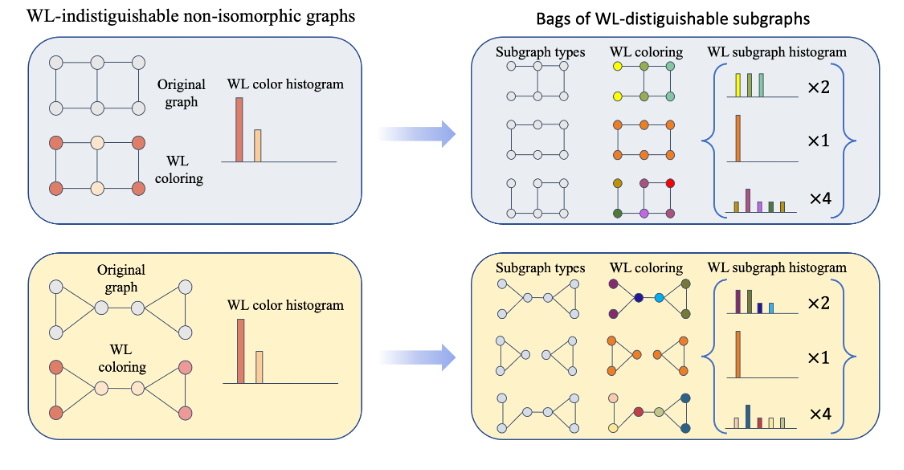
\includegraphics[width=.80\textwidth]{figures/Expressive_Power.png}
    \caption{\textbf{Left:} WL Graph isomorphism incapable of distinguishing a basic pair of graphs. \textbf{Right:} Bags of Sub-graphs computed using Edge-Deleted policy, which can distinguish the two graphs successfully. From \cite{beatrice_esan_2021}.}
    \label{fig:expressive_power_wl_esan}
\end{figure}
\subsection{Definitions}
\begin{definition}[Graphs]
\label{def:graph_def}
Graphs with $n$ vertices are defined as $G=(A,X)$. Here, $A\in\mathbb{R}^{n\times n}$ is the graph's Adjacency matrix and $X\in\mathbb{R}^{n\times d}$ is node feature matrix (each node feature vector is of dimension $d$).
\end{definition}
\begin{definition}[Neighbourhood]
\label{def:neighbourhood_def}
The neighbourhood of a vertex $V$, in a Graph $G$ is a subgraph containing nodes that are adjacent to $V$ or that are connected to $V$ directly and all the edges connecting them. 
\end{definition}
\begin{definition}[Mutliset or Bags of subgraphs]
A Bag or Multiset of subgraphs is defined by \emph{S\textsubscript{G} = $\{\!\!\{G\textsubscript{1},.\ .\ .,G\textsubscript{m}\}\!\!\}$}. Here $G$ is the original graph and it can be represented by a multiset ($S_G$) of its constituent subgraphs $G_1,...,G_m$.
\label{def:multiset_bag}
\end{definition}
\begin{definition}[Symmetric Group]
This report will be introducing two type of Symmetric group, \textit{Subgraph Symmetry}, $S_n$ and \textit{Set Symmetry}, $S_m$. $S_n$ in the is a multiset of all the permutations of nodes in a graph. And $S_m$ is the permutation of all subgraphs in a multiset or bags of Subgraphs ($S_G$ - See above definition). 
\end{definition}
\begin{definition}[Isomorphic Graphs]
\label{def:isomporphism}
Two Graphs $G_1$ and $G_2$ are isomorphic if,
\begin{enumerate}
    \item The number of edges and vertices in both graphs are same.
    \item The edge connectivity of both graphs is same.
\end{enumerate}
\end{definition}
\begin{definition}[Weisfeiler-Lehman Test]
\label{def:wl_test}
The Weisfeiler-Lehman Isomorphism Test (WL) \citep{weisfeiler_1968} is a hierarchy of polynomial-time algorithms for determining if graphs are isomorphic. The k-WL test iteratively recolors k-tuples of vertices of a graph at each step as per some neighborhood aggregation rules. It stops once we reach a stable coloring.
\end{definition}
\begin{definition}[Graph neural networks]
\label{def:gnn} 
Graph Neural Networks (GNN), are a class of neural networks that process graph data. Message Passing Neural Network (MPNN) \citep{gilmer_mpnn_2017} is one of the popular architecture under GNN. MPNN are defined by several message passing layers, which is expressed in \citep{christopher_higher_order_gnn_2019} as,\begin{center}
    \emph{ \[ x\rlap{\textsubscript{v}}\textsuperscript{t} = W\rlap{\textsubscript{1}}\textsuperscript{t}\hspace{1mm}x\rlap{\textsubscript{v}}\textsuperscript{t-1} + W\rlap{\textsubscript{2}}\textsuperscript{t}  \sum_{u\sim v} x\rlap{\textsubscript{u}}\textsuperscript{t-1}+b\textsuperscript{t} \]}
\end{center}
Here, \emph{x\rlap{\textsubscript{v}}\textsuperscript{t}} is the feature of node v after the application of t\textsuperscript{th} layer, \emph{W\textsubscript{i}, b} are the learn-able parameters and v are all the nodes in the neighbourhood of u. 
\end{definition}
\begin{definition}[Expressive power of GNNs] \label{def:expressive_gnn} 
It defines the ability of a GNN model to distinguish non-isomorphic graphs.
\end{definition}
\begin{definition}[Symmetry Group and Group actions]
\label{def:symm_gp_actions}
\cite{GeometricDL_Bronstein_2021} introduced the concept of \textit{Geometic Priors} according to which an input, for example an image or a graph, is a signal in some \emph{domain} $\Omega$, a 2-Dimensional Grid (See Figure \ref{fig:geometric_priors}). The \emph{symmetry group} $\mathfrak{G}$, describes the structure of the domain, $\Omega$, that is all the permutations of the input. For example a set of all 2D translations for an input image. The elements of the group, is referred as Group actions (\emph{$\mathfrak{g}\in\mathfrak{G}$}), for example a group action is one of the element in a set of all 2D translations of an input image. \emph{Symmetry group} is defined by \emph{Group representation}, $\rho(\mathfrak{G})$ in signal space $\mathcal{X}(\Omega)$.
\end{definition}
\begin{definition}[Invariance and equivariance] \label{def:inv_equiv} 
\textbf{Invariant} functions are the ones that are not affected by the action of a group, i.e.,
$f(\rho(\mathfrak{g})x)=f(x)$ for any $g\in\mathfrak{G}$. Contrastingly, in \textbf{Equivariant} functions the output is transformed in the same way as the input, i.e., $f(\rho(\mathfrak{g})x)=\rho(\mathfrak{g})f(x)$ for any $g\in\mathfrak{G}$.
\end{definition}
\subsection{Limitations of MPNNs}\label{sec:limit_MPNN}
\citep{christopher_higher_order_gnn_2019} and \citep{xu_power_nn_2019} presented analysis on the expressive power of MPNNs. The study concluded that MPNNs despite all thier populairty are at most as expressive as the $1$-WL Graph isomorphism test. Moreover, the study states that, WL test cannot distinguish simple pair of graphs as shown in Figure \ref{fig:expressive_power_wl_esan}. This inspired a quest for lot of new GNN algorithms with improved expressive power.
\begin{figure}
    \centering
    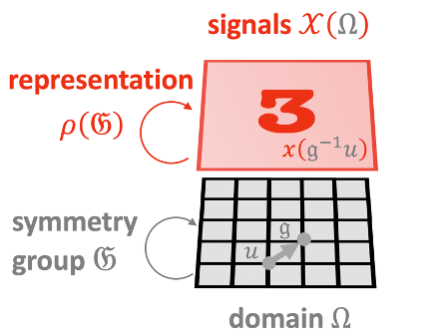
\includegraphics[width=.50\textwidth]{figures/geometric_priors.png}
    \caption{Illustrations of Geometric Deep Learning: \emph{signal space} $\mathcal{X}(\Omega)$, \emph{domain} $\Omega$, Symmetries of the domain $\Omega, $ given by group $\mathfrak{G}$, acts on signals $x\in\mathcal{X}(\Omega)$ through group representations $\rho(\mathfrak{g})$, restricts the structure of hypothesis class. From \cite{GeometricDL_Bronstein_2021}.}
    \label{fig:geometric_priors}
\end{figure}
\subsection{Other Powerful Architectures}
There have been several recent works that proposed some powerful architectures with better expressiveness then MPNNs. \\ One of the method is \emph{k}-WL tests (\citep{christopher_higher_order_gnn_2019}, \citep{christopher_gosparse_2020}) which is compromise between expressivity and complexity. However, it gets really difficult to implement anything above 2nd order networks. Other possible approaches involves using structural encoding for nodes and edges with standard MPNN method. Other alternative approaches includes MPNNs with structural encodings for nodes and edges (for example, clique or cycle counts) \citep{bouritsas_improv_gnn_2022} or lift graphs into cell complexes \citep{bodnar_weisfeiler_cw_2021a}. Though, there is a pre-computation step for all these approaches which may get very expensive.

\section{ESAN Framework}
In contrast to MPNN, \citep{beatrice_esan_2021} proposes \emph{Equivariant Subgraph Aggregation Networks} (ESAN), which has better expressive power. Finding distinguishable subgraphs between two distinct graphs is at the core of this approach. Similar to WL test which encodes multiset of \emph{node colors}, ESAN opts for encoding bags of subgraphs. Each graph is represented as a bag or multiset of its subgraph. The subgraphs are chosen by some predefined policy, such as removing an edge from the graph, as illustrated in Figure \ref{fig:expressive_power_wl_esan}.
\\The framework constitutes of the following,
\begin{enumerate}
    \item Architecture to process multi-set of sub-graphs
    \item Sub-graph Selection Policies
\end{enumerate}
\subsection{Bag of Graphs Encoder Architecture}
This section outlines a Neural Network Architecture for processing multi-sets of subgraphs to produce a final graph representation. \citep{beatrice_esan_2021} presents an equivariant architecture called DSS-GNN as well its variant DS-GNN. 

\begin{figure}
    \centering
    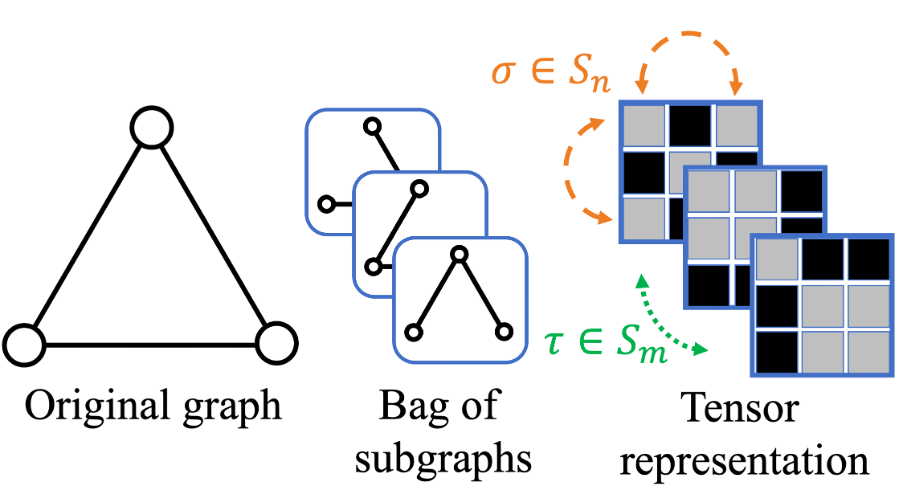
\includegraphics[width=.50\textwidth]{figures/symmetries.png}
    \caption{Symmetry Structure of subgraphs using edge deletion policy and m = 3. The subgraphs are represented by \textit{m$\times$n$\times$n} tensor $\mathcal{A}$. \textit{$\sigma \in S\textsubscript{m}$} permutes on nodes of subgraphs and \textit{$\tau \in S\textsubscript{n}$} permutes on the subgraphs. From \cite{GeometricDL_Bronstein_2021}.}
    \label{fig:symmetries}
\end{figure}

\subsubsection{Symmetry group for sets of graphs}
The bags of sub-graphs of \emph{G}, \emph{S\textsubscript{G}} (with \emph{n} nodes and \emph{m} subgraphs) can be represented as \emph{$(\mathcal{A,X})\in\mathbb{R}$\textsuperscript{n$\times$n$\times$m}$\times\mathbb{R}$\textsuperscript{n$\times$d$\times$m}}, here \emph{$\mathcal{A}\in\mathbb{R}$\textsuperscript{n$\times$n$\times$m}} corresponds to \emph{m} Adjacency matrices and \emph{$\mathcal{X}\in\mathbb{R}$\textsuperscript{n$\times$d$\times$m}} is a set of \emph{m} feature matrices for \emph{m} subgraphs and $d$ is the length of node feature vector.\\
\emph{Subgraph symmetries} which is the permutation of nodes in the original graph, is represented by symmetric group S\textsubscript{n}. And it acts on \textit{(A,X)} as following,
\begin{center}
    \emph{$(\sigma$$\cdot$A)\textsubscript{ij}=A\textsubscript{$\sigma$\textsuperscript{-1}(i)$\sigma$\textsuperscript{-1}(j)}} and \emph{$(\sigma$$\cdot$X)\textsubscript{il}=X\textsubscript{$\sigma$\textsuperscript{-1}(i)l}}, \textit{$ \sigma \in S\textsubscript{n}$}
\end{center}
The permutation of Subgraphs in S\textsubscript{G}, which is \textit{set symmetries}, given by symmetric group  S\textsubscript{m} and it acts on \textit{$\mathcal{(A,X)}$} as,
\begin{center}
    \emph{$(\tau$$\cdot\mathcal{A}$)\textsubscript{ijk}=$\mathcal{A}$\textsubscript{$ij\tau$\textsuperscript{-1}(k)}} and \emph{$(\tau$$\cdot\mathcal{X}$)\textsubscript{ilk}=$\mathcal{X}$\textsubscript{il$\tau$\textsuperscript{-1}(k)}}, \textit{$ \tau \in S\textsubscript{m}$}
\end{center}
\textit{Subgraph Symmetry} and \textit{Set Symmetry} are combined into a single Group, $H=\left(S_n\times S_m\right)$ as in Figure \ref{fig:symmetries}. It acts on $\mathcal{(A,X)}$ as following, \begin{center}
    $
((\tau, \sigma) \cdot \mathcal{A})_{i j k}=\mathcal{A}_{\sigma^{-1}(i) \sigma^{-1}(j) \tau^{-1}(k)}, \quad((\tau, \sigma) \cdot \mathcal{X})_{i l k}=\mathcal{X}_{\sigma^{-1}(i) l \tau^{-1}(k)}
$
\end{center}
To put it simply, $\sigma$ permutes the nodes and $\tau$ permutes the subgraphs. Moreover, same permutation $\tau$ is applied over all subgraphs, thus nodes are ordered consistently over all subgraphs.

\subsubsection{H-equivariant Layers}
\begin{figure}
    \centering
    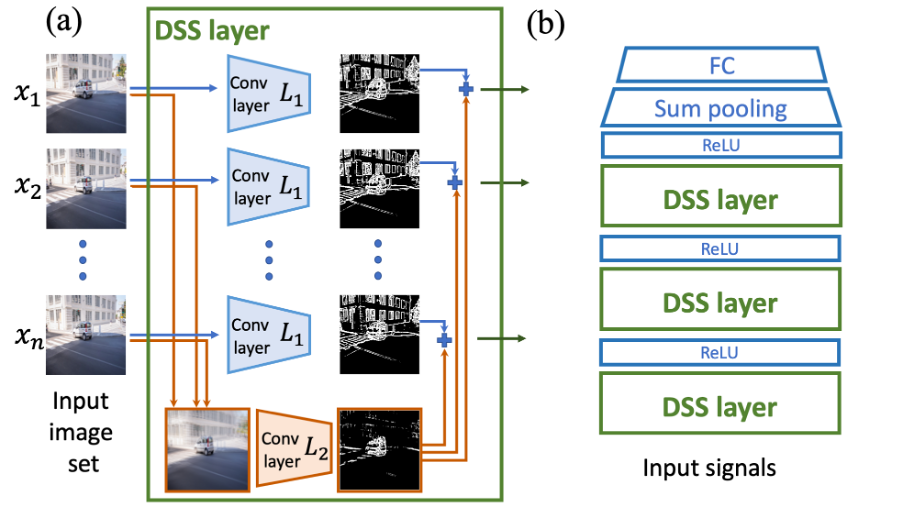
\includegraphics[width=.80\textwidth]{figures/dsslayer.png}
    \caption{A DSS layer is composed of a Siamese Component (blue) that is applied to each component individually and an aggregation module (orange), that sums up all the images. The output of aggregation module is added to the Siamese output part. From \cite{haggai_symlearning_2020}.}
    \label{fig:dsslayer}
\end{figure}
Equivariant architectures process subgraph bags in accordance with their natural symmetry (Product of \textit{set} and \textit{subgraph} symmetry). Building blocks of such an architecture are H-equivariant layers. \citep{haggai_symlearning_2020} presented a method for learning sets of symmetric elements. The approach involves defining the symmetric group for the sets of symmetric elements, then defining the linear layer space that corresponds to it. It is composed of a Siamese component applied to each element individually, and an information sharing module that aggregates all elements. A simple DSS layer on a set of images is illustrated in Figure \ref{fig:dsslayer}.\\
Motivated by this approach, \cite{beatrice_esan_2021} adopted the same layer structure (Figure \ref{fig:h_equiv_layer}) composed of a Siamese and an information sharing component and parameterized it using an equivariant GNN layer like MPNN. The Layer ($L: \mathbb{R}^{n \times n \times m} \times \mathbb{R}^{n \times d \times m} \rightarrow \mathbb{R}^{n \times n \times m} \times \mathbb{R}^{n \times d^{\prime} \times m}$) takes in a bag of subgraphs and outputs another bag of subgraphs.
\begin{center}
$(L(\mathcal{A}, \mathcal{X}))_i=L^1\left(A_i, X_i\right)+L^2\left(\sum_{j=1}^m A_j, \sum_{j=1}^m X_j\right)$
\end{center}
Here, $(L(\mathcal{A}, \mathcal{X}))_i$ is the output of \textit{i}-th subgraph when applied to the layer, $L^1, L^2$ $: \mathbb{R}^{n \times n} \times \mathbb{R}^{n \times d} \rightarrow \mathbb{R}^{n \times n} \times \mathbb{R}^{n \times d^{\prime}}$ represents two base graph encoders. By parametrizing $L^1, L^2$ with MPNN the adjacency matrix of the processed subgraphs remain same, i.e., \textit{H}-equivariany layer outputs the same adjacency matrix along with the processed nodes features.\\
While $L^1$ treats each graph independently, $L^2$ allows information to be shared across all subgraphs. DSS presented in \citep{haggai_symlearning_2020}, uses a sum aggregator, given by 
$\left(\sum_{j=1}^m A_j\right.$ and $\left.\sum_{j=1}^m X_j\right)$. Although other aggregator can be used such as mean, max or aggregator that without the applied subgraph, i.e., $\left(\sum_{j \neq i}^m A_j\right.$ and $\left.\sum_{j \neq i}^m X_j\right)$. Eventually, the \textit{$S_n$} equivariance of base encoder and \textit{$S_m$} equivariance of the aggregator gives \textit{H}-equivariance (see Figure \ref{fig:h_equiv_layer}) of the layer. 
\begin{figure}
    \centering
    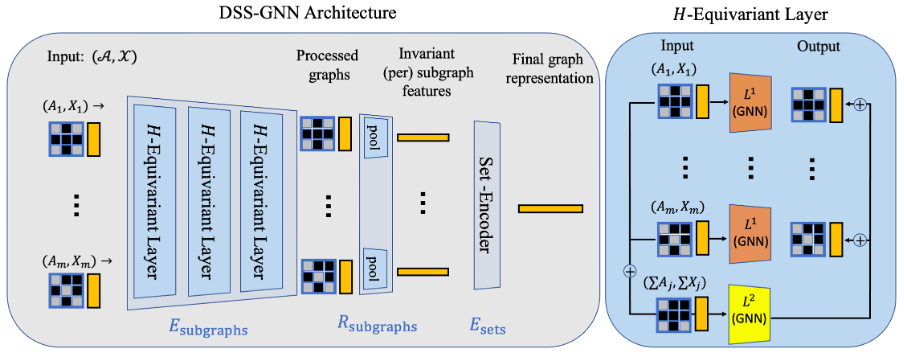
\includegraphics[width=.90\textwidth]{figures/Hequivlayer.png}
    \caption{\textbf{Left}: DSS-GNN architecture, composed of a Feature Encoder, a Readout Layer and a Set Encoder. \textbf{Right}: An H-equivariant Layer with  a Siamese component (Orange) and an information-sharing (yellow). From \cite{beatrice_esan_2021}.}
    \label{fig:h_equiv_layer}
\end{figure}

\subsubsection{DSS-GNN}
The DSS-GNN (illustrated in Figure \ref{fig:h_equiv_layer}) is an architecture based on the DSS-GNN layer. It comprises of three parts and they are put together as follows,
\begin{equation} \label{eq:dss_gnn_equation}
        F_{\text {DSS-GNN }}=E_{\text {sets }} \circ R_{\text {subgraphs }} \circ E_{\text {subgraphs }}
\end{equation}
\begin{itemize}
    \item \emph{Equivariant feature encoder (E\textsubscript{subgraphs}}) : $\mathbb{R}^{n \times n \times m} \times \mathbb{R}^{n \times d \times m} \rightarrow$ $\mathbb{R}^{n \times n \times m} \times \mathbb{R}^{n \times d' \times m} $ \\
    It consist of several \textit{H}-equivariant layers and it learns useful features for the nodes in all of the applied sugraphs.
    \item \emph{Subgraph Readout Layer R\textsubscript{subgraphs}} : $\mathbb{R}^{n \times n \times m} \times \mathbb{R}^{n \times d' \times m} \rightarrow$ $\mathbb{R}^{d' \times m} $ \\
    This part creates a invariant feature vector by aggregating node  and edge features independently for each input subgraph.
    \item \emph{Universal Set Encoder E\textsubscript{sets}} : $\mathbb{R}^{d' \times m} \rightarrow$ $\mathbb{R}^{d''} $ \\
    It outputs a final vector graph representation using a universal set encoder such as DeepSets \citep{zaheer_deepsets_2017} or PointNet \citep{qi_pointnet_2017}.
\end{itemize}
(E\textsubscript{subgraphs}$\circ$R\textsubscript{subgraphs}) encodes a subgraph to a \textit{$S_n$}-invariant representation and E\textsubscript{sets} produces a single \textit{H}-invariant representation corresponding to the original Graph, \textit{G} from a set of \textit{$S_n$}-invariant subgraphs.


\subsubsection{DS-GNN}
It is a variant of DSS-GNN, in which information sharing component of each  \emph{H-equivariant layer of E\textsubscript{subgraphs}} is set to off. We set \textit{$L^2=0$} in equation \ref{eq:dss_gnn_equation} for each of the layer in E\textsubscript{subgraphs}. Thus, there is no information sharing component, each subgraph is encoded independently. In this arrangement, all the subgraphs are aligned, that is they have the same node permutation.

\subsection{Subgraph Selection Policies}
In this section we discuss the various subgraph selection policies that effect the expressive power of our architecture.\\
Some basic notation,
\begin{itemize}
    \item \textit{G}: Set of all graphs with n or less nodes.
    \item $\mathbb{P}(G)$: Set of all subsets, $S \subseteq G$.
    \item $\pi$: Its the Subgraph selection policy, it assigns a set of subgraphs for each Graph, \textit{G}. The subgraph selection should be invariant of the node permutation.
\end{itemize}
We use this notation $\pi(G)\coloneqq S^\pi_G$. Here, the order of subgraph is arbitrary but the order of nodes within each subgraph is same.\\
The paper defined following subgraph selection policies,
\begin{itemize}
    \item \textbf{Node-Deleted Policy}: Set of sub-graphs obtained by removing an edge from the original Graph.
    \item \textbf{Edge-Deleted Policy}: Removing a single edge.
    \item \textbf{EGO-Networks Policy}: Maps original graph to a set of ego-networks of some depth \emph{k}, one for each node in the graph.
    \item \textbf{EGO+ Network Policy}: Variant of EGO where the root node has a identifying feature.
    \item \textbf{Augmented Policy $\hat{\pi}$} : Adding original graph to bag of sub-graphs obtained by using any selection policy $\pi$, to ensure at least the expressive power of the basic graph encoder. We donate any of the above subgraph selection policy as augmented policy by introducing a hat over the policy name, for example an Augmented EGO-Network policy is denoted by $\widehat{EGO}$.
\end{itemize}
\subsubsection{Stochastic Sampling} Using entire bag of subgraphs might prove expensive for larger graphs. We use stochastic sampling as solution to this. It selects a small subset, $|\Bar{S^\pi_G}|\subset S^\pi_G$ uniformly and randomly for every training epoch.

\section{Computational Complexity}In this section we analyse the complexity of ESAN, table \ref{tab:complexity_analysis} summarizes the results for ESAN and some other known models.\begin{table}[h!]
    \centering
    \begin{tabular}{c | c c}
    \hline
    Model & Time & Space \\
    \hline\\
    PPGN & $\mathcal{O}\left(n^3\right)$ & $\mathcal{O}\left(n^2\right)$\\\\
    3-IGN & $\mathcal{O}\left(n^3\right)$ & $\mathcal{O}\left(n^3\right)$\\\\
    3-GNN & $\mathcal{O}\left(n^4\right)$ & $\mathcal{O}\left(n^3\right)$\\\\
    GSN & $\mathcal{O}\left(n\Delta_{max}\right)$ & $\mathcal{O}\left(n+n \Delta_{\max }\right)$\\\\
    CWN & $\mathcal{O}\left(\sum_{p=1}^2 n_p\left(B_p+2\left(\begin{array}{c}B_p \\2\end{array}\right)\right)\right)$ & $\mathcal{O}\left(n+ \sum_{p=1}^2 n_p\left(1+B_p+2\left(\begin{array}{c}B_p \\2\end{array}\right)\right)\right)$\\\\
    \hline\\
    \textbf{ESN} & $\mathcal{O}\left(|S| n \Delta_{\max }\right)$ & $\mathcal{O}\left(|S|\left(n+n \Delta_{\max }\right)\right)$\\\\
    \hline
    \end{tabular}
    \caption{Complexity of Graph Networks. $\Delta_{max}$ denotes maximum degree over all nodes. From \cite{beatrice_esan_2021}}
    \label{tab:complexity_analysis}
\end{table}
\subsection{Time Complexity}ESAN requires $\mathcal{O}\left(|S|n^2\right)$ time, here each subgraph is processed using MPNN which has a time complexity of $\mathcal{O}\left(n^2\right)$. For node-deleted and ego-net subgraph selection policies, $|S|=\mathcal{O}\left(n\right)$, that results in a total time complexity of $\mathcal{O}\left(n^3\right)$, which is equal to PPGN \citep{haggai_provab_powerfulgnn_2019a} and 3-IGN \citep{haggai_inv_equiv_2019b}. Furthermore, for edge-deleted graph selection policies, $|S|=\mathcal{O}\left(n^2\right)$, that gives a total time complexity of $\mathcal{O}\left(n^4\right)$, which is comparable to 3-GNN \citep{christopher_higher_order_gnn_2019}.\\
For sparse Graphs the time complexity of ESAN improves to $\mathcal{O}\left(|S|n\Delta_{max}\right)$, here $\Delta_{max}$ is maximum node degree. Relative to PPGN and k-IGN this is a major benefit for ESAN, as the former two do not improve for sparse graphs. For sparse graph $\Delta_{max}=1$.\\
Table \ref{tab:complexity_analysis} also present two sparse architechtures, GSN \citep{bouritsas_improv_gnn_2022} and CWN \citep{bodnar_weisfeiler_cw_2021a}. GSN gives the same complexity as of standard GNNs for small number of subgraphs. ESAN can match complexity of GSN, only in the case when stochastic sampling used. However, the prepossessing phase for GSN is expensive. For CWN, time complexity is given by a general lifting procedure that generate two dimensional cellular complex. $n_p$ denotes the number of cells at dimension p and $B_p$ is the maximum boundary size. The number of nodes is given by $n_0 = n$ and number of edges by $n_1=\mathcal{O}\left(n\Delta_{max}\right)$. The complexity of CWN is given by, $\mathcal{O}\left(n\Delta_{max}+n_2\right)$.  In a general graph distribution, the number of 2-cells may grow exponentially, however $n_2$ is contained in case of molecules.
\subsection{Space Complexity} Time complexity of ESAN is given by $\mathcal{O}\left(|S|\left(n+n\Delta_{max}\right)\right)$, which includes computing $n$ node features, by keeping track of subgraph connectivity. Therefore, the complexity is $\mathcal{O}\left(n^2\Delta_{max}+\left(n\Delta_{max}\right)^2\right)$ for edge-deleted policy and $\mathcal{O}\left(n^2+n^2\Delta_{max}\right)$ for node-deleted and ego-net subgraph selection policies. However for DS-GNN architechture the space complexity improves to $\mathcal{O}\left(n+n\Delta_{max}\right)$. Subgraph selection policies like low depth ego-net policies has lesser number of edges, which means smaller subgraph sizes thus they have increased efficiency.
\subsection{Preprocessing}
Applying subgraph selection policy to generate subgraphs from the Original Graph $G$, is a one time work and done before the training. Node Deleted and Edge deleted subgraph selection policies takes $\mathcal{O}\left(nm\right)$ and $\mathcal{O}\left(m^2\right)$ respectively, here $n$ is the number of nodes and $m$ is number of edges. Moreover, for sparse graphs, m can have a upper bound of $\mathcal{O}\left(n\Delta_{max}\right)$, where $\Delta_{max}$ is usually small for sparse graphs. Ego-Net policy takes $\mathcal{O}\left(n\left(n+m\right)\right)$, which includes $\mathcal{O}\left(n+m\right)$ for breadth first search, to compute the k-neighbourhood of a node. Furthermore, the runtime complexity might get significantly reduced for sparse graphs.
\section{Theoretical Analysis}
In this section we examine the expressive power of our architecture. We introduce a WL analogues for ESAN and analyse how different design choices affects the expressiveness of ESAN.
\subsection{WL Analogue for ESAN}
The paper introduced two refinement procedures, \textbf{DSS-WL} and its variant \textbf{DS-WL} that encodes bags of sub-graphs, inspired by the WL isomorphism test \citep{weisfeiler_1968}. The idea is that a pair of graphs are more effectively separated by encoding subset of their contained subgraphs rather than encoding the nodes of the graphs as done in WL isomorphism test.
Below is a description of the procedure.
\subsubsection{Initiation} The DSS-WL takes in as input, the pair of graphs $G^1$, $G^2$ and a subgraph selection policy, $\pi$. First, the algorithm applies the subgraph selection policy and generates subgraphs from the original graphs. Then each node in each subgraph is assigned a color based on the initial coloring (if provided) or randomly.
\subsubsection{Refinement} The color of the node, $v$ in a subgraph $S$ is refined according to the formula$\colon$
\begin{center}
    $c_{v,S}^{t+1} \leftarrow$ HASH$\left(c_{v,S}^t,N^t_{v,S},C^t_v,M^t_v\right)$ 
\end{center}
Here, $N^t_{v,S}$ is multiset of colors in $v$'s neighbourhood in a subgraph $S$, $C^t_v$ is multiset of $v$'s colors across all subgraphs and $M^t_v$ is a multiset of aggregated colors of $v$'s neighbourhood across all subgraphs according to the original graph connectivity.
\subsubsection{Termination}The subgraph $S$ in each step of the algorithm is associated with a color $c_s$, which is a multiset of color associated with the nodes in the subgraph. So, each graph is represented by multisets of subgraphs colors. As soon as the multisets start to diverge the algorithm terminates and the graphs are concluded to be non-isomorphic. However, if the refinement step assigns same representation two both graphs, the test is inconclusive.\\
DS-WL is a variant of DSS-WL where the refinement rule does not consider input $C^t_v$ and $M^t_v$. That is the inputs representing information sharing across subgraphs is disabled, which results in a vanilla WL that runs on each subgraph independently.
\subsection{WL Analogue and Expressive Power}
The paper presents couple of results (for proof refer to the main paper) regarding the expressive power of the DSS-WL.\\\\
\textbf{Theroem 1}: DS(S)-WL is strictly more powerful than 1-WL. \\
The idea behind this is, that there exists subgraph selection policies such that,
\begin{enumerate}
    \item Any pair of graphs that is distinguishable by WL is also distinguished by DS(S)-WL.
    \item There exists pairs of graphs which are distinguishable by DS(S)-WL but cannot be distinguished by WL. Circulant Skip Link graphs (see definition below) is an example of such graph pairs.
\end{enumerate}\textbf{Circulant Skip Link graphs:} As defined in \cite{murphy_rel_pooling_2019}, Circulant Skip Link, CSL(M, R) represents an undirected 4-regular graph(degree of all nodes is 4) with vertices $\{0, 1, . . . , M − 1\}$ whose edges form a cycle and have skip links. Here, $R$ and $M$ are co-prime such that $R<M-1$, for cycle $\{j,j+1\}\inE, j\in\{0,1,M-2\}$ and $\{M-1,0\}\inE$ and for skip links, we recursively define a sequence $s_1=0$, $s_{i+1}=(s_i+R)\mod M$ and $\{s_i,s_{i+1}\}\inE$ for $i\in\mathbb{N}$.
\\\\The paper presents the below result, which proves that DS(S)-WL is able to distinguish such pairs of CSL graphs (See Figure \ref{fig:expressive_power_wl_esan} for example of ESAN with CSL using Edge Deleted subgraph selection policy).\\\\
\textbf{Lemma 1} CSL$(n, 2)$ \textit{can be distinguished from any CSL}$(n, k)$ \textit{with} $k\in[3,n/2-1]$ \textit{by} \textit{DS-WL} \textit{and} \textit{DSS-WL} \textit{with either the} ND, EGO, or EGO+ policy.\\\\
Furthermore, the paper present this result which shows that the expressive power of our variants can be attained by ESAN.\\\\
\textbf{Theorem 2} DSS-GNN at least as powerful as DS(S)-WL; DS-GNN at most as powerful as DS-WL.\\ \textit{Let $\mathcal{F}$ be any family of bounded-sized graphs endowed with node labels from a finite set. There exist selection policies such that, for any two graphs $G^1,G^2$ in $\mathcal{F}$, distinguished by DS(S)-WL, there is a DS(S)-GNN model in the form of Equation (\ref{eq:dss_gnn_equation}) assigning $G^1,G^2$ distinct representations. Also, DS-GNN with MPNN base graph encoder is at most as powerful as DS-WL.}\\\\
The above theorem is valid until each egde that exists in original graph appears at least once in any of the subgraphs. Following this assumption, DS(S)-GNN has a power at least equal to DS(S)-WL. In conjunction with Theorem 2, we can therefore conclude that there are policies for subgraph selection that make ESAN more powerful than WL.\\
Furthermore, the paper presents the following corollary based on  results of \citep{xu_power_nn_2019} and \citep{christopher_higher_order_gnn_2019} (MPNN being at most as stronger as WL test) and Theorem 1, Theorem 2.\\\\
\textbf{Corollary 1} (DS(S)-GNN is strictly more powerful than MPNNs). \textit{There exists subgraph selection policies such that DSS-GNN and DS-GNN architectures are strictly more powerful than standard MPNN models in distinguishing non-isomorphic graphs.}

\subsection{Expressiveness of Design Choices}
This section analyses various significant design choices for ESAN. 
\subsubsection{DSS vs DS matters} DSS-GNN performs as well or better than DS-GNN, depending on the subgraph selection policy.
\subsubsection{Base graph encoder} A DSS-GNN with either of depth-l $\widehat{EGO}$ or $\widehat{EGO}+$ as subgraph selection policy and a 3-WL base graph encoder is strictly powerful than 3-WL and a DSS-GNN with 3-WL base graph encoder more powerful than the one with 1-WL base graph encoder. That is, ESAN gains expressiveness by increasing the expressive power of the graph encoder.
\subsubsection{Subgraph selection policy} The significance of Subgraph selection policy in respect to expressive power can be explained through Strongly Regular (SR) Graphs.SR graphs are defined by 4 parameters ($n,k,\lambda,\mu$). 1-WL and 3-WL cannot distinguish SR graphs with same parameters. A DS-GNN with ND, EGO+ or ED subgraph policy can easily distinguish SR graphs with different parameters. However, it cannot distinguish SR graphs with same parameters just like 1-WL and 3-WL. Moreover, a DSS-GNN with ED policy can distinguish some SR graphs with same parameters. Thus for SR graphs, DS-GNN with ND, EGO are as strong as 3-WL test and DS-GNN with ED is more powerful than 3-WL.
\section{Experiments}
In this section we test ESAN on several data-sets and compare the results with base graph encoders. We run tests with different combinations of sub-graph selection policies, the two variants DSS-GNN and DS-GNN, full approach or stochastic variant, to compare the expressive power of various combinations.
\begin{itemize}
    \item \textbf{EXP, CEXP, CSL}: On these datasets, results shows that 1-WL GNN, GIN and Graphconv performs no better than a random guess. However, ESAN gives perfect accuracy with either of 1-WL, GIN or Graphconv base encoders. Moreover, even stochastic variants gives similar accuracy. 
    \item \textbf{TUDatasets}: On TUDatasets SoTA method outperforms all other methods. However, reports excellent results right behing SoTA. ESAN outperforms other methods such as ID-GNN and RNI. The results shows that, particularly successful configurations are:
    \begin{enumerate}
        \item DSS-GNN (EGO+) + GraphConv/GIN
        \item DS-GNN (ND) + GIN
    \end{enumerate}
    Moreover, analysis of results also tells stochastic variant is a strong alternative for base encoder based methods. 
    \item \textbf{OGB}: On OGB dataset all ESAN variants  outperforms their base encoder GIN. Furthermore, DSS-GNN performs better that DS-GNN with GCN base encoder.
    \item \textbf{ZINC12K}: Results show that all variants of ESAN outperforms their base GIN encoder. However, in general ESAN performs competitively with other method irrespective of selected subgraph policies. It outperforms PNA model. However other methods are only outperformed when ESAN is equipped with EGO(+) policy.
\end{itemize}

\section{Conclusion}
The paper presented a novel framework, ESAN, with increased expressiveness over its former counterpart like MPNN and performs significantly good with several graph classification benchmarks. Though, ESAN is more computationally expensive then MPNN, and the paper also describes a stochastic version to alleviate this problem.

\setcitestyle{numbers}
\bibliography{bibliography}
\end{document}
